\documentclass[a4paper,10pt]{article}
\usepackage[utf8]{inputenc}
\usepackage[T1]{fontenc}
\usepackage[francais]{babel}
\usepackage{lmodern}
\usepackage{geometry}
\geometry{a4paper, margin=1in}
\usepackage{enumitem}
\usepackage{graphicx} % Pour inclure la photo
\usepackage{hyperref}
\usepackage{fancyhdr}
\usepackage{multicol}
\usepackage{array}
\usepackage{xcolor}

% Configuration de la page

\begin{document}

% Header amélioré avec photo
\begin{tabular}{>{\bfseries}l c l}
    \begin{minipage}{0.7\textwidth} % Largeur du texte (à gauche)
        \textbf{\LARGE DEMUTH AXEL} \\[0.3cm]
        \textbf{Mail:} axeldemuth67150@gmail.com \\[0.1cm]
        \textbf{Téléphone:} +33 07 71 08 67 12 \\[0.1cm]
        \textbf{GitHub:}Ademuth \\
        Strasbourg, France
    \end{minipage} &
    \begin{minipage}{0.3\textwidth} % Largeur de la photo (à droite)
        \raggedleft % Aligner à droite
        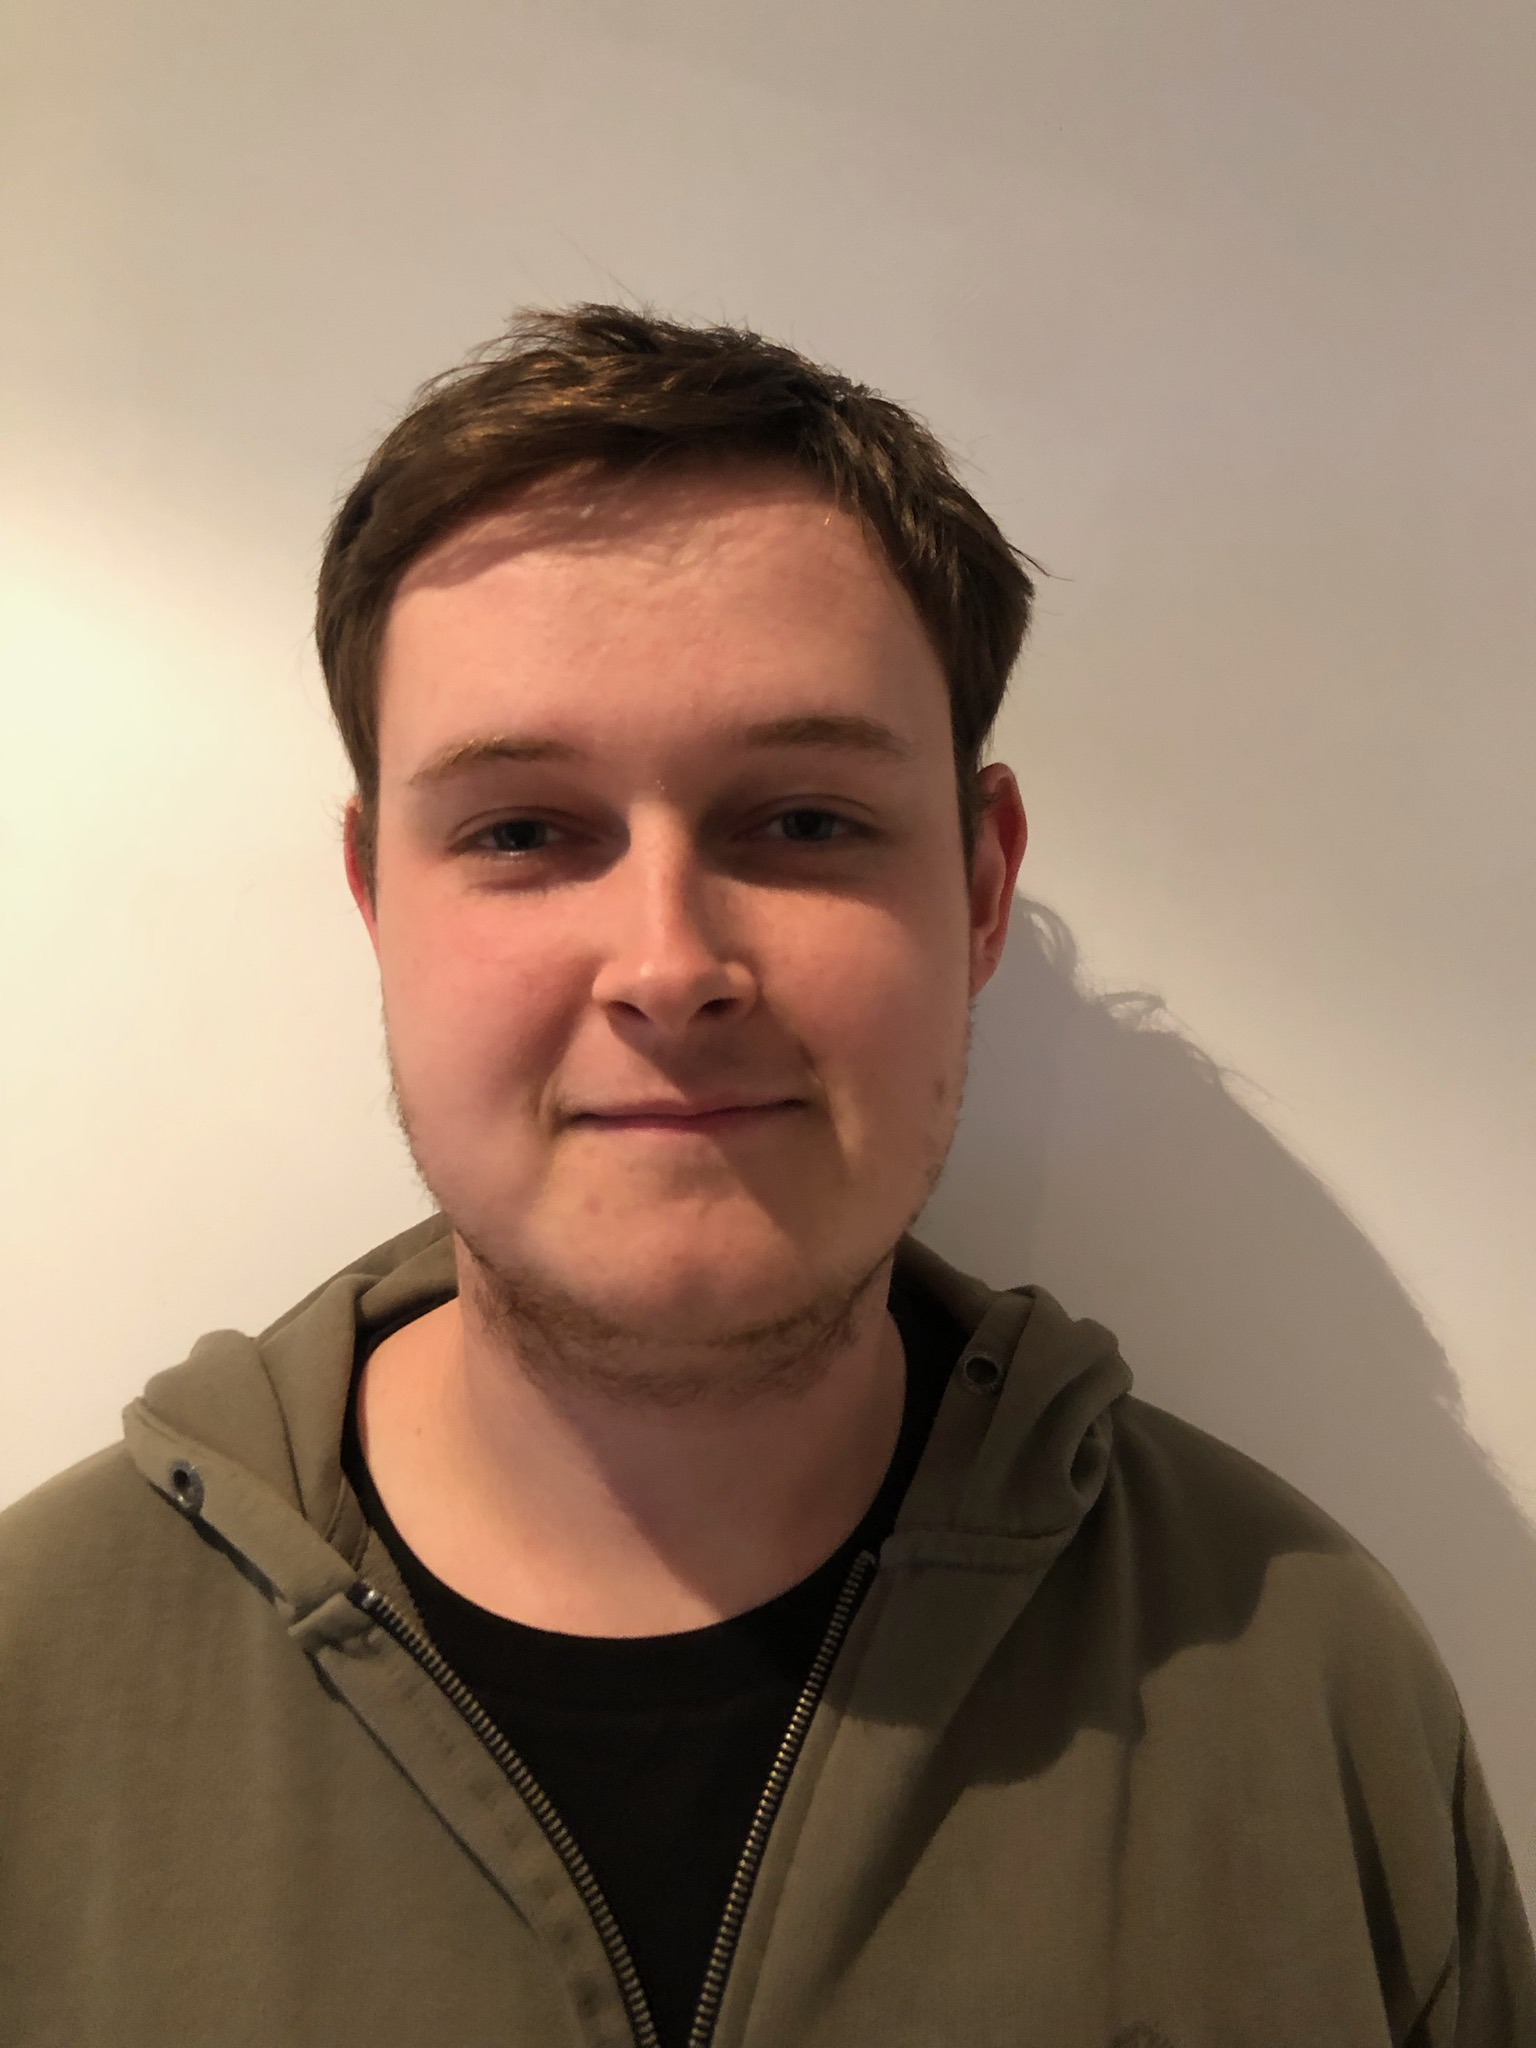
\includegraphics[width=3.5cm]{photo.jpg} % Inclure votre photo (ajustez la taille selon vos besoins)
    \end{minipage}
\end{tabular}

\vspace{0.5cm}

% Ajout de l'objectif de stage
\begin{center}
    \textbf{À la recherche d'un stage de M2 d'une durée de 4 à 6 mois entre février et août 2025}
\end{center}

\vspace{0.5cm}

\section*{Formation}
\noindent
\textbf{Master en Mathématiques Appliquées} \\
Université de Strasbourg, 2023 - en cours \\
Spécialisation en calcul scientifique et mathématiques de l'innovation, avec des compétences en simulation, modélisation et data science. \\

\noindent
\textbf{Principales matières:} Analyse fonctionnelle, Optimisation, Équations aux dérivées partielles (EDP), Intelligence artificielle (IA), Calcul haute performance (HPC), Analyse de signal, Analyse de graphes. \\
\noindent
\textbf{Langages de programmation:} Python, C++, C, Julia. \\

\noindent
\textbf{Bibliothèques:} CGAL,MPI,STL,Tensorflow,Pytorch,Sklearn,Scipy,Pandas,Plotly
\vspace{0.2cm}

\noindent
\textbf{Licence en Mathématiques et Informatique} \\
Université de Strasbourg, 2019 - 2023 \\
\noindent
\textbf{Cours suivis :} Algèbre, Calcul différentiel, Probabilités, Statistiques, Équations différentielles ordinaires (EDO), Analyse de Fourier, Programmation en Python et C++. \\

\vspace{0.1cm}

\noindent
\textbf{Langues} \\
\textbf{Français :} Natif, \textbf{Anglais :} Niveau B2


\vspace{0.2cm}

\section*{Expériences}
\noindent
\textbf{Stage - IRMA Strasbourg} \\
Juin à août 2024 \\
Développement d'une bibliothèque pour le projet Ktirio Urban Building dans le cadre du projet Numpex Exa-MA. Contribution au module Kinetic, en utilisant la bibliothèque CGAL et l'algorithme de reconstruction de surface cinétique pour reconstruire des maillages 3D à partir de nuages de points, avec correction des imprécisions du maillage. \\

\vspace{0.3cm}

\noindent
\textbf{Projet - Simulation de la chaleur sur un CPU} \\
Réalisation d'une simulation en C++ du comportement thermique d'un CPU à l'aide de solutions numériques d'EDP. Implémentation de deux modèles : stationnaire et dynamique. \\

\vspace{0.3cm}

\noindent
\textbf{Emplois étudiants}
\begin{itemize}
    \item Équipier polyvalent, McDonald's Erstein, été 2023
    \item Livreur de journaux, DNA, été 2022
\end{itemize}

\end{document}
